\lecture{2}{jeu 20 fev 2020}
\vspace{-1.2cm}

\section{Évolution de la publicité}

\epigraph{We are facing our Kodak moment; a point of inflection \\ where we can choose between two future states: \\ reinvention or the long march into irrelevance.}{\textit{Gareth Kay, Cannes Lions 2013}}

Dans un séminaire organisé lors du festival Cannes Lions en 2013, Gareth Kay fait cet appel au monde de la publicité: il faut faire une transition urgente vers le digital.\\

Avant, la publicité était passive et consommée dans des endroits ou pendant des activités spécifiques: le salon (devant sa télé), en lisant le journal ou un magasine, dans la rue (panneaux publicitaires), etc. Ce nombre réduit de médiums était contraignant, car il apportait des limitations au niveau du processus créatif. Par exemple, le format des encarts ou panneaux publicitaires est souvent très réglementé (rectangulaire, taille fixe, endroit précis), tout comme la longueur d'un spot publicitaire télévisé. Ceci avait pour implication de mettre au coeur du processus créatif la trouvaille d'un concept qui devait être un message très simple et facile à comprendre, choisir le ou les médias à explorer (la plupart étant payants et très chers), puis impliquer les spécialistes (graphistes, vidéastes, etc) vers le milieu/fin du processus. \\

Aujourd'hui, la trouvaille d'un concept accrocheur reste primordiale, mais il ne s'agit plus juste d'un message à transmettre, mais aussi du moyen par quel le faire atteindre le public cible, car les formats possibles sont beaucoup plus nombreux. Il faut créer tout un écosystème, en partant du storytelling, tout en étant hyper réactif et à l'écoute des nouvelles ou trends actuelles ("social listening"). Les spécialistes doivent donc être intégrés dans le processus dès le début, pour analyser les possibilités et limites de la campagne, et créer une stratégie digitale solide et cohérente. Les rôles évoluent aussi: on ne trouve plus seulement que des créatifs et des spécialistes en marketing dans les équipes, mais aussi des développeurs, des maquettistes, des vidéastes, etc. Il faut aussi être attentif à la plateforme que l'on utilise, car chacune d'elles a ses codes, son langage et sa façon de communiquer propre.\\

\begin{figure}[H]
\hspace{-0.5cm}
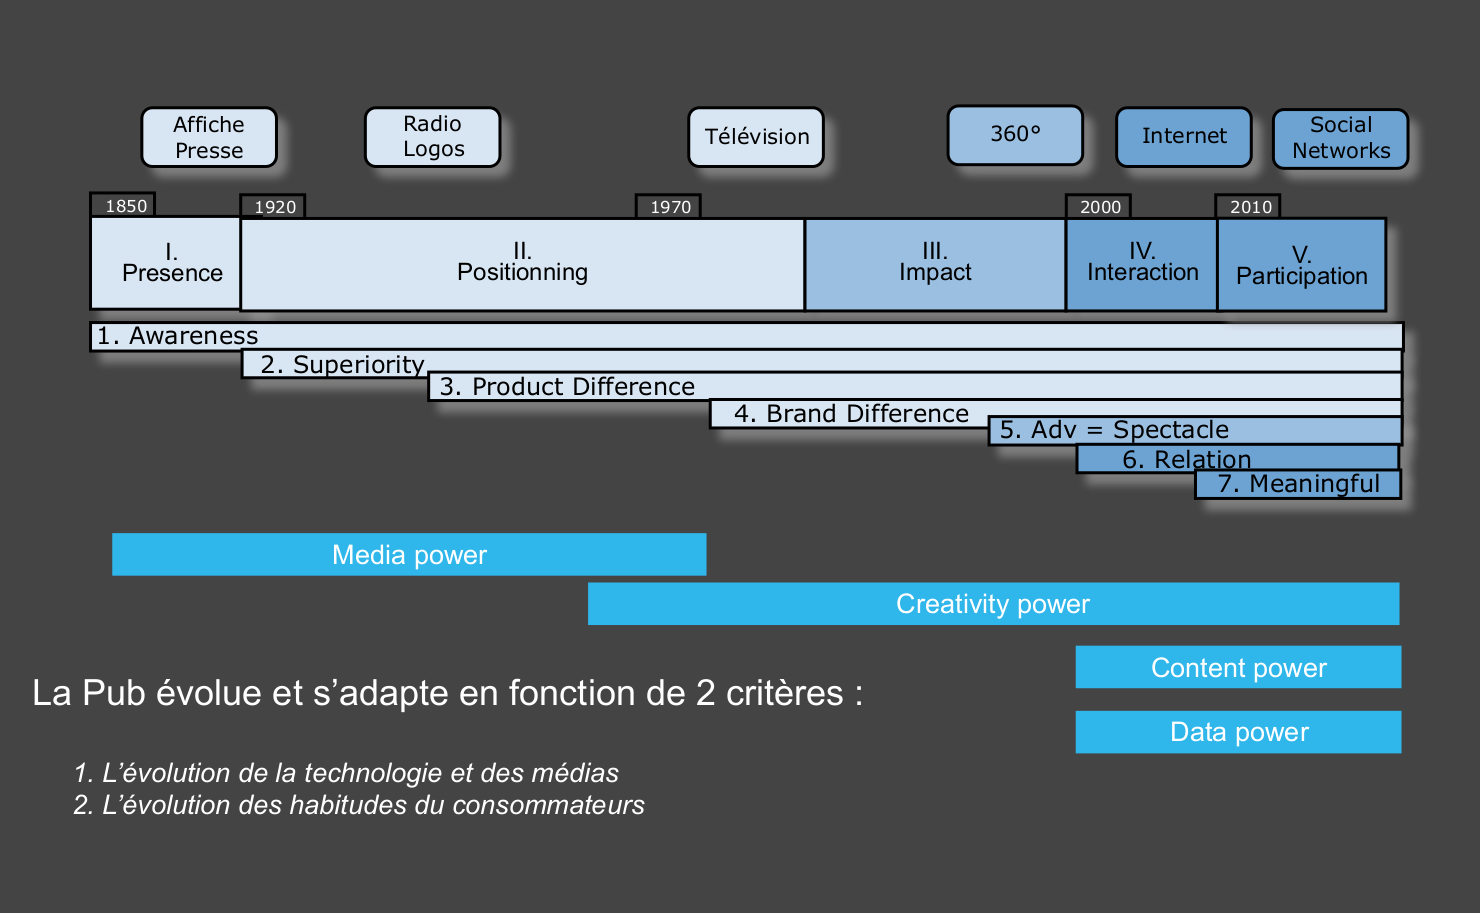
\includegraphics[scale=0.30]{../images/lec2img1}
\end{figure}

Il y a deux raisons principales à ce besoin de changement drastique d'approche: Premièrement, l'évolution de la technologie et l'explosion des types de médias différents apportent un florilège de nouveaux médiums, qui ne restreignent plus les créateurs de campagnes marketing à, par exemple, une affiche publicitaire standard ou un carré aux tailles hyper formatées dans un journal. Deuxièmement, les moeurs et les habitudes du consommateur ont changé. Outre le fait que la plupart des consommateurs ont pris l'habitude d'ignorer la plupart des formats standards de publicité, il y a eu aussi une montée du pouvoir du bouche à oreille. Ils préfèrent écouter l'avis d'autres consommateurs avant de se faire une idée. \\

Ceci a mené à trois évolutions majeures, que l'on va analyser dans les prochains sous-chapitres: les meaningful brands, la coach attitude, et le participative marketing.

\subsection{Meaningful brands}

\epigraph{We live in a world of content overload. (...) In this world, only brands \\that form more meaningful connections with people will prosper.}{\textit{Yannick Bolloré, CEO of Havas Group}}

Dans le passé, les publicités avaient pour but premier de démontrer les avantages fonctionnels d'un produit (prix, caractéristiques, avantages). Par la suite, le but est devenu aussi de se démarquer et montrer en quoi la marque est meilleure que ses compétiteurs (Functional / Cost-Advantage \& Aspirational / Differentiation).\\

À présent, dans un monde où il y a une avalanche journalière de contenu et de publicité, et étant donné que les moeurs du consommateur ont changé (comme dit précédemment), le public est beaucoup plus à l'écoute de la responsabilité sociétale de la marque.\\

Les trois piliers principaux des meaningful brands:

\begin{itemize}
    \item \textbf{Personal benefits:} Le produit est bon pour vous, il améliore votre qualité de vie et vous allez vous sentir mieux après l'avoir acheté (santé, condition physique, financière, intellectuelle, sociale, émotionnelle);
    \item \textbf{Collective benefits:} L'entreprise qui produit ce produit a un impact sociétal positif (éthique, communautaire, écologique ou autres);
    \item \textbf{Functional benefits}: Vous avez besoin du produit car il fonctionne et délivre un service qui est très utile.\\
\end{itemize}

\begin{center}
\resizebox{0.95\textwidth}{!}{
    \begin{tikzpicture}
\coordinate (A) at (-5,0) {};
\coordinate (B) at ( 5,0) {};
\coordinate (C) at (0,5) {};
\draw[name path=AC] (A) -- (C);
\draw[name path=BC] (B) -- (C);
\foreach \y/\A in {0/Product Attributes (differentiating),1/Functional Benefits,2/Emotional Benefits,3/Values} {
    \path[name path=horiz] (A|-0,\y) -- (B|-0,\y);
    \draw[name intersections={of=AC and horiz,by=P},
          name intersections={of=BC and horiz,by=Q}] (P) -- (Q)
        node[midway,above] {\A};
}
\end{tikzpicture}

}
\end{center}

\newpage

\subsection{Coach Attitude}

\epigraph{We are not in the businness of supporting a media industry, \\we are in the business of connecting with customers.}{\textit{Trevor Edwards, VP Nike, 2007}}

\vspace{-0.5cm}

L'exemple de Nike est l'illustration parfaite de la marque coach. Depuis de nombreuses années, leur communication est centrée sur des messages qui visent à booster leurs consommateurs et les pousser à faire de l'exercice (en achetant de préférence, bien sur, leurs produits). Depuis leur tagline ("Just do it.") à leurs applications de tracking sportif, en passant par des campagnes vidéos, la marque se positionne totalement dans cette attitude de coach.\\

Les marques coach ont donc, dans leur marketing, moins de focus sur les produits mais plus sur les personnes qui les utilisent. Elles aident leurs clients, en leur donnant des outils pour, à se fixer des objectifs (qu'ils soient de santé, carrière, scolaires, beauté, etc). Elles doivent donc se doter de trois caractéristiques:

\begin{itemize}
    \item \textbf{Se fixer un objectif:} Sorte de promesse classique réinventée, elle inscrit la marque dans une recherche de mieux-être spécifique et incarnée.
    \item \textbf{Se doter d'une personnalité:} À l'instar d'un coach, qui dispose d'une personnalité, d'une posture vis-à-vis de ses coachés, la marque doit faire ce même cheminement.
    \item \textbf{Proposer des outils:} Pour sortir de la pensée magique et de la promesse sans soutien, ce qui rend une marque coache, ce sont les outils, le programme qu'elle est à même de proposer pour coacher ses consommateurs.\\
\end{itemize}

Deux postures différentes peuvent être adoptées: \textbf{Enabler} (booste, dicte, surveille, tire vers le haut, incite à se surpasser ou \textbf{Mentor} (conseille, suggère, aide, soutient, compatit).\\

Avec l'avènement du digital, de nouvelles modalités relationnelles peuvent se créer avec le consommateur. On distingue 5 leviers du digital au service du coaching:

\begin{itemize}
    \item \textbf{Plus d'accessibilité:} smart devices, internet
    \item \textbf{Plus de récurrence et de rapidité:} emails, newsletters, notifications, réseaux sociaux, applications mobiles
    \item \textbf{Plus d'intelligence collective:} crowdsourcing, crowdfunding, plateformes collectives
    \item \textbf{Plus de connaissance et de personnalisation:} avoir plus d'informations sur le consommateur grâce aux données et aux appareils connectés
    \item \textbf{Plus de dialogue:} chat, social media \\
\end{itemize}

Avec ces caractéristiques, postures et outils, on a distingué par la suite plusieurs approches marketing lorsqu'on veut se positions comme une marque coache:

\begin{itemize}
    \item \textbf{Coacher par le contenu:} Présenter au quotidien du contenu récurent sur une thématique précise, afin d'accompagner le client sur la durée avec des conseils qui vont lui permettre de s'améliorer.
    \item \textbf{Coacher par le programme:} Comme le précédent, mais avec un programme personnalisé conçu selon les besoins de chacun.
    \item \textbf{Coacher par la donnée:} Surveiller les performances et booster les clients sur base de données collectées, afin de les accompagner de façon ultra personnalisée.
    \item \textbf{Coacher par la communauté:} Utiliser les réseaux sociaux afin d'établir une relation conversationnelle avec ses clients et les accompagner au quotidien de façon proche.
    \item \textbf{Coacher par le jeu:} Inciter ses consommateurs à atteindre leurs objectifs en leur fixant des challenges via une dynamique de Gamification (voir chapitre 3).
    \item \textbf{Coacher dans la réalité:} Soutenir dans la vraie vie en organisant des rencontres IRL, afin de prolonger la relation et le coaching.
    \item \textbf{Coacher par le concours:} Offrir des plateformes qui permettent de mettre sur le devant de la scène des gens avec des talents, afin d'élire les meilleurs et ensuite les coacher pour booster leur carrière.\\
\end{itemize}
